\chapter{\label{cha:sts_introduction}Introduction}

Semantic Textual Similarity (STS), measures the equivalence of meanings between two textual segments. In Natural Language Processing (NLP), measuring semantic similarity between two textual segments plays an important role and one of the fundamental tasks for many NLP applications and its related areas. To measure STS, the input is always two textual segments and the output is a continues value that represents the degree of similarity of the two input textual segments. 


STS is related to both textual entailment (TE) and paraphrasing, but differs in a number of ways. TE can draw three directional relationships between two text fragments while the task considered two text fragments as text (t) and hypothesis (h) respectively. On the other hand, paraphrasing identification is the task of recognising text fragments with approximately the same meaning within a specific context. Therefore, TE and paraphrasing gives a categorical output while STS identifies the degree of equivalence of texts as a continues value. 

 Measuring STS is an important research problem, having many applications in NLP such as information retrieval (IR) \cite{10.1145/1097047.1097051, 5571521}, text summarisation \cite{ALIGULIYEV20097764, SCHALLEHN2004361}, question answering \cite{mohler-etal-2011-learning}, relevance feedback \cite{WANG2020102342}, text classification \cite{10.1007/978-3-642-41278-3_74, 10.1007/978-3-319-11749-2_8} and word sense disambiguation \cite{10.1007/978-3-642-17432-2_44}. In the field of databases, text similarity can be used for schema matching. In the document databases like Elasticsearch\footnote{Elasticsearch is a document database based on the Lucene library. It is available on \url{https://www.elastic.co/}. More information on Similarity module is available on \url{https://www.elastic.co/guide/en/elasticsearch/reference/current/index-modules-similarity.html}}, there is a core module called \textit{"Similarity module"} that defines the document matching process. Furthermore, STS is also useful for relational join operations in databases where join attributes are textually similar to each other \cite{10.1145/352595.352598, SCHALLEHN2004361}. Also, STS is widely used in semantic web applications like community extraction \cite{10.1007/978-3-642-14589-6_33}, Twitter search \cite{feng-etal-2013-twitter} where it is required the ability to accurately measure semantic relatedness between concepts or entities.
 
 These applications require to measure STS automatically which means that computer programs should be developed to calculate STS between two textual inputs. This can be considered as a Machine Learning (ML) problem. Over the years, researchers have proposed numerous ML solutions for STS. These ML solutions can be categorised in to two main categories;  
 \begin{enumerate*}[label=(\alph*)]
 	\item Linguistic feature based
 	\item Vector/ Embedding based
 \end{enumerate*}
. Most of the early approaches belong to linguistic feature based category. With this, features to the ML algorithm were hand-crafted. Such features include edge-distances between nodes in WordNet \cite{10.1145/219717.219748}, number of named entities in two input texts, corpus pattern analysis features etc. Then these features would be fed in to a ML algorithm such as Support Vector Machine (SVM), Linear Regression etc \cite{bechara-etal-2015-miniexperts}. This ML algorithm will be trained on an annotated STS dataset and then can be used to measure STS automatically. Despite being extremely popular before the neural network era, linguistic feature based algorithms have limitations. Determining the best linguistic features for calculating STS is not an easy task as it requires a good understanding of the linguistic phenomenon and relies on researchers' intuition. In addition, most of these features depend on lexical knowledge-bases like WordNet, which makes it difficult to adopt them in languages other than English. However, the biggest limitation of these methods would be, they no longer provide strong results compared to the vector based methods. 

With the introduction of word embeddings \cite{DBLP:journals/corr/abs-1301-3781}, ML solutions in NLP shifted from feature based methods to vector based methods. Pre-trained word embedding models provide a learned representation for texts where the words that have the same meaning have a similar representation. Since these word embeddings are already semantically powerful, ML solutions no longer requires to depend on lexical knowledge-bases. As a result, embedding based ML solutions are easy to adopt in different languages as long as the pre-trained embeddings are available in that language. Furthermore, these solutions are now the state-of-the-art in NLP tasks including STS too providing stronger results than feature based ML solutions. Therefore, as STS solutions in this part of the thesis,  we mainly explore embedding based ML approaches.

Similar to general ML algorithms, vector based ML STS algorithms can too be classified in to two main categories; Supervised and Unupervised. In supervised learning, ML models will be trained using labelled data. It means that data is already annotated by the humans with the correct answer. For unsupervised learning, you do not need an annotated dataset. Unsupervised ML approach would discover features by itself. Given that annotated STS data is not commonly available in many languages and domains it is important to explore both supervised and unsupervised STS methods. Therefore, first two chapters in this part of the thesis explore unsupervised STS methods while the last two chapters in this part explore supervised STS methods. 

Most common unsupervised STS approaches are vector aggregation methods like Word Vector Averaging, Word Mover's Distance \cite{10.5555/3045118.3045221} and Smooth Inverse Frequency \cite{DBLP:conf/iclr/AroraLM17}. In Chapter \ref{cha:sts_state_of_the_art_methods} we explore them in detail. We identify the best vector aggregation method empirically by analysing them in different STS datasets and finally we propose a new state-of-the-art vector aggregation method based on contextual word embeddings that outperforms other methods. 

In Chapter \ref{cha:sts_sentence_encoders} we explore another unsupervised STS method using sentence encoders. Sentence encoders are different from vector aggregation methods as they have end-to-end models to get sentence embeddings rather than a simple aggregation method. They provide strong results compared to other unsupervised STS methods. We use three different sentence encoders and analyse their performance in various aspects of English STS and also evaluate their portability to different languages and domains. 


In Chapter \ref{cha:sts_siamese_neural_networks} and \ref{cha:sts_transformers} we explore most popular supervised STS approaches. Usually, in supervised vector based STS approaches, word embeddings would be fed in to a neural network. There are popular neural network structures when it comes to STS. Tree-structured neural networks \cite{tai-etal-2015-improved} and Siamese neural networks are such structures \cite{Mueller_Thyagarajan_2016}. Among them Siamese neural networks have been widely used in STS and has additional advantages compared to other structures. Therefore, we discuss them comprehensively in Chapter \ref{cha:sts_siamese_neural_networks}. We evaluate the existing Siamese Neural Network architectures in STS datasets and propose a novel Siamese Neural Network architecture for smaller STS datasets that outperforms current state-of-the-art Siamese neural models.  We also asses its performance on different languages and domains.

In the final chapter of the Part I of this thesis, we explore the newly released transformers in STS tasks. Transformers have taken NLP field by storm providing very successful results in variety of NLP tasks. In Chapter \ref{cha:sts_transformers}, we bring together various transformer architectures like BERT \cite{devlin-etal-2019-bert}, XLNet \cite{yang2019xlnet}, RoBERTa \cite{liu2019roberta} etc and investigate their performance in various STS datasets. We explore the strengths and weaknesses of transformer models regarding the accuracy and efficiency and discover the possible solutions for its limitations.

The main contributions of this part of the thesis are as follows.

\begin{enumerate}
	\item In each chapter, we cover various supervised and unsupervised techniques to compute semantic similarity that can benefit a wide range of NLP application. We empirically evaluate all of them in three English datasets, two non English datasets and an out of domain dataset to explore their adaptability. 
	
	\item We propose a novel unsupervised STS method based on contextual word embeddings that outperforms current state-of-the-art unsupervised vector aggregation STS methods in all the English datasets, non-English datasets and datasets in other domains. 
	
	\item We propose a novel Siamese neural network architecture which is efficient and outperforms current state-of-the-art Siamese neural network architectures in smaller STS datasets. 
	
	\item We provide important resources to the community. The code of the each chapter as an open-source GitHub repository and the pre-trained STS models will be freely available to the community. The link to the GitHub repository and the models will be unveiled in the introduction section of the each chapter. 
\end{enumerate}

The remainder of this chapter is structured as follows. Section \ref{sec:sts_intro_datsets} discuss the various datasets we used in \textit{"Semantic Textual Similarity"} part of the thesis. We also briefly analyse the datasets for common properties. In Section \ref{sec:sts_evaluation} we discuss the main evaluation metrics we used in the \textit{"Semantic Textual Similarity"} part of the thesis. Chapter concludes with the conclusions.


\section{Datasets}
\label{sec:sts_intro_datsets}
The popularity of STS is partially owed to the large number of shared tasks organised in SemEval from 2012-2017 \cite{agirre-etal-2012-semeval,agirre-etal-2013-sem,agirre-etal-2014-semeval,agirre-etal-2015-semeval,agirre-etal-2016-semeval,cer-etal-2017-semeval}. First, they have provided annotated datasets which can be used to train STS ML models and to evaluate them. Second, at the end of each shared task, the solutions submitted by the participants are published and the best solutions can be considered as state-of-the-art STS methods. 

We experimented with several datasets throughout the experiments in the Semantic Textual Similarity Section that has been released for these shared tasks. In order to maintain the versatility of our methods we experimented with several English STS datasets as well as several non English datasets and a dataset from a different domain which we will discuss later in this section. These datasets carry different interesting characteristics. Therefore, with the introduction we also do an exploratory analysis of the dataset focussing on different properties of the dataset. All of the datasets which are described here are publicly available and can be considered as STS benchmarks. 

\subsection{English Datasets}
\begin{enumerate}
  \item \textbf{SICK dataset} \footnote{The SICK dataset is available to download at \url{https://wiki.cimec.unitn.it/tiki-index.php?page=CLIC}} - The SICK data contains 9927 sentence pairs with a 5,000/4,927 training/test split which were employed in the SemEval 2014 Task1: Evaluation of Compositional Distributional Semantic Models on Full Sentences through Semantic Relatedness and Textual Entailment \cite{marelli-etal-2014-semeval}. The dataset has two types of annotations: Semantic Relatedness and Textual Entailment. We only use Semantic Relatedness annotations in our research. SICK was built starting from two existing datasets: the 8K ImageFlickr data set \footnote{The 8K ImageFlickr data set is available at \url{http://hockenmaier.cs.illinois.edu/8k-pictures.html}} \cite{rashtchian-etal-2010-collecting} and the SemEval-2012 STS MSR-Video Descriptions dataset \footnote{The SemEval-2012 STS MSR-Video Descriptions dataset is available at \url{https://www.cs.york.ac.uk/semeval-2012/task6/index.html}} \cite{agirre-etal-2012-semeval}. The 8K ImageFlickr dataset is a dataset of images, where each image is associated with five descriptions. To derive SICK sentence pairs the organisers randomly selected 750 images and sampled two descriptions from each of them. The SemEval2012 STS MSR-Video Descriptions data set is a collection of sentence pairs sampled from the short video snippets which compose the Microsoft Research Video Description Corpus \footnote{The Microsoft Research Video Description Corpus is available to download at \url{https://research.microsoft.com/en-us/downloads/38cf15fd-b8df-477e-a4e4-a4680caa75af/}}. A subset of 750 sentence pairs have been randomly chosen from this data set to be used in SICK. 
  
  In order to generate SICK data from the 1,500 sentence pairs taken from the source data sets, a 3-step process has been applied to each sentence composing the pair, namely \textit{(i) normalisation, (ii) expansion and (iii) pairing} \cite{marelli-etal-2014-semeval}. The \textit{normalisation} step has been carried out on the original sentences to exclude or simplify instances that contained lexical, syntactic or semantic phenomena such as named entities, dates, numbers, multiword expressions etc. In the \textit{expansion} step syntactic and lexical transformations with predictable effects have been applied to each normalised sentence, in
  order to obtain \textit{(i)} a sentence with a similar meaning, \textit{(ii)} a sentence with a logically contradictory or at least highly contrasting meaning, and \textit{(iii)} a sentence that contains most of the same lexical items, but has a different meaning. Finally, in the \textit{pairing} step each normalised sentence in the pair has been combined with all the sentences resulting from the expansion phase and with the other normalised sentence in the pair. Furthermore, a number of pairs composed of completely unrelated sentences have been added to the data set by randomly taking two sentences from two different pairs \cite{marelli-etal-2014-semeval}. 
  
  Each pair in the SICK dataset has been annotated to mark the degree to which the two sentence meanings are related (on a 5-point scale). The ratings 
  have been collected through a large crowdsourcing study, where each pair 
  has been evaluated by 10 different annotators. Once all the annotations were collected, the relatedness gold score has been computed for each pair as the average of the ten ratings assigned by the annotators \cite{marelli-etal-2014-semeval}. Table \ref{tab:sickdata} shows examples of sentence pairs with different degrees of semantic relatedness; gold relatedness scores are expressed on a 5-point rating scale. Given a test sentence pair the machine learning models require to predict a value between 0-5 which reflects the relatedness of the given sentence pair. 
  
  \begin{table}[ht!]
  	\centering 	
  	\begin{tabular}{l|c} 
  		\hline
  		\multicolumn{1}{c|}{\textbf{Sentence Pair}} & 
  		\multicolumn{1}{c}{\textbf{Relatedness}}  \\
  		\hline
  		\makecell[l]
  		{1. A little girl is looking at a woman in costume. \\ 
  		 2. A young girl is looking at a woman in costume.} & 4.7  \\
  		\hline
  			\makecell[l]
  		{1. Nobody is pouring ingredients into a pot. \\ 
  			2. Someone is pouring ingredients into a pot. } & 3.5  \\
  		\hline
  		\makecell[l]
  		{1. Someone is pouring ingredients into a pot. \\ 
  		 2. A man is removing vegetables from a pot. } & 2.8  \\
  		\hline
  		\makecell[l]
  		{1. A man is jumping into an empty pool. \\ 
  		 2. There is no biker jumping in the air. } & 1.6  \\
  		\hline               
  	\end{tabular}
  	\caption[Example sentence pairs from the SICK dataset]{Example sentence pairs from the SICK dataset with their gold relatedness scores (on a 5-point rating scale). \textbf{Sentence Pair} column shows the two sentence and \textbf{Relatedness} column denotes the annotated relatedness score.}
  	\label{tab:sickdata}
  \end{table}

Figure \ref{fig:sick_relatedness} shows the distribution of the relatedness value in SICK training and SICK testing set. It is clear that there are more sentence pairs with a high relatedness values compared to low relatedness values. SICK train and SICK test follows a similar distribution. 


\begin{figure}
	\captionsetup[subfigure]{justification=centering}
	\centering
	\begin{subfigure}[b]{.5\textwidth}
		\centering
		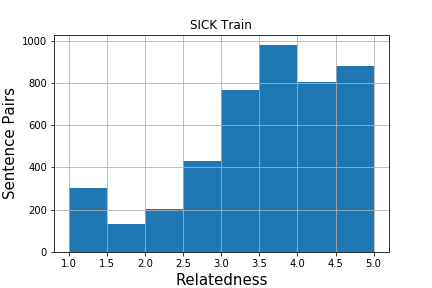
\includegraphics[width=\textwidth]{figures/semantic_textual_similarity/introduction/sick_train_relatedness_hist.png}
		\caption{Relatedness distribution of \\ SICK training test}
		\label{fig:sick_train_relatedness}
	\end{subfigure}%
	\begin{subfigure}[b]{.5\textwidth}
		\centering
		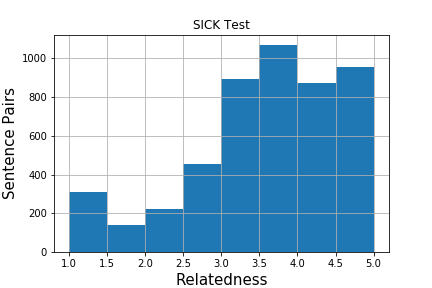
\includegraphics[width=\textwidth]{figures/semantic_textual_similarity/introduction/sick_test_relatedness_hist.png}
		\caption{Relatedness distribution of \\ SICK testing set}
		\label{fig:sick_test_relatedness}
	\end{subfigure}
	\caption[Relatedness distribution of SICK train and SICK test]{Relatedness distribution of SICK train and SICK test. \textit{Sentence Pairs} shows the number of sentence pairs that a certain \textit{Relatedness bin} has.}
	\label{fig:sick_relatedness}
\end{figure}


\begin{figure}
	\captionsetup[subfigure]{justification=centering}
	\centering
	\begin{subfigure}[b]{.5\textwidth}
		\centering
		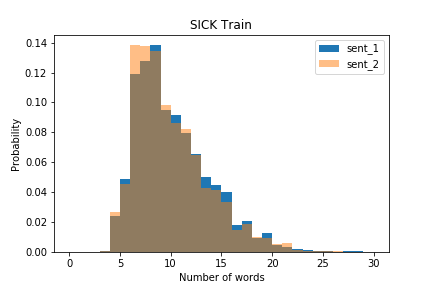
\includegraphics[width=\textwidth]{figures/semantic_textual_similarity/introduction/sick_train_words.png}
		\caption{Normalised distribution of word count in SICK train}
		\label{fig:sick_train_words}
	\end{subfigure}%
	\begin{subfigure}[b]{.5\textwidth}
		\centering
		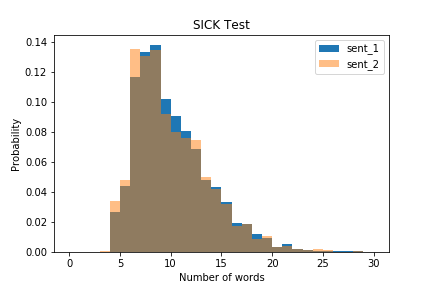
\includegraphics[width=\textwidth]{figures/semantic_textual_similarity/introduction/sick_test_words.png}
		\caption{Normalised distribution of word count in SICK test}
		\label{fig:sick_test_words}
	\end{subfigure}
	\caption[Normalised distribution of word count in SICK train and SICK test.]{Normalised distribution of word count in SICK train and SICK test. \textit{Number of words} indicates the word count and \textit{Probability} shows the total probability of a sentence with that word count appearing in the dataset.}
	\label{fig:sick_words}
\end{figure}


\begin{table*}
	\centering
	\begin{tabular}{l|cc|cc}
		\hline
		Measure   & \multicolumn{2}{c|}{SICK Train} & \multicolumn{2}{c}{SICK Test} \\
		\hline
		\multicolumn{1}{l|}{} & \textbf{Sent$\_$1} & \textbf{Sent$\_$2} & \textbf{Sent$\_$1} & \textbf{Sent$\_$2} \\
		\textit{Word Count Mean} & 9.73 & 9.52 & 9.69 & 9.53  \\
		\textit{Word Count STD} & 3.66 & 3.70 & 3.69 & 3.65  \\
		\textit{Word Count MAX} & 28 & 32 & 28 & 30  \\
		\textit{Word Count MIN} & 3 & 3 & 3 & 3  \\
		\hline
	\end{tabular}
	\caption[Word count stats in SICK]{Word count stats in SICK training and SICK testing. \textit{STD} indicates the standard deviation and the other acronyms indicate the common meaning }
	\label{table:sick_sts}
\end{table*}

In Figure \ref{fig:sick_words} we visualise the normalised distribution of word count for both sentence 1 and sentence 2 in SICK train and SICK test. Both sentences have a similar distribution reaching the maximum around 9 words. SICK train and SICK test follows a similar pattern in word count distribution too. Additionally we show some word count statistics in Table \ref{table:sick_sts}. In SICK train number of words for a sentence ranges from 3 to 32 and have the mean number of words around 9.5. These statistics are extremely close in SICK test too. 


\begin{figure}
	\captionsetup[subfigure]{justification=centering}
	\centering
	\begin{subfigure}[b]{.5\textwidth}
		\centering
		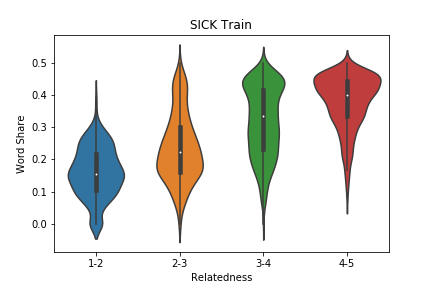
\includegraphics[width=\textwidth]{figures/semantic_textual_similarity/introduction/sick_train_word_share.png}
		\caption{Word share against relatedness bins in SICK train}
		\label{fig:sick_train_word_share}
	\end{subfigure}%
	\begin{subfigure}[b]{.5\textwidth}
		\centering
		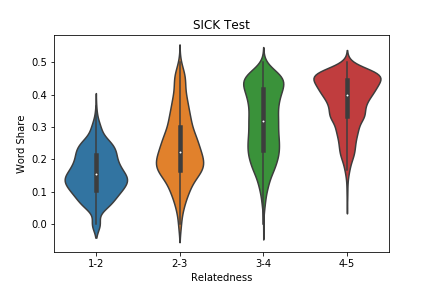
\includegraphics[width=\textwidth]{figures/semantic_textual_similarity/introduction/sick_test_word_share.png}
		\caption{Word share against relatedness bins in SICK test}
		\label{fig:sick_test_word_share}
	\end{subfigure}
	\caption[Word share against relatedness bins in SICK train and SICK test.]{Word share against relatedness bins in SICK train and SICK test. \textit{Word Share} indicates the ratio between number of common words in the two sentences to total number of words in the two sentences against each \textit{Relatedness} bins}
	\label{fig:sick_word_share}
\end{figure}

The common judgement in STS is that, when two sentences share a large number of words, the relatedness of that two sentences should be higher. In fact, in early feature based approaches of calculating semantic textual similarity, the number of overlapping words between the two sentences was a common feature \cite{vilarino-etal-2014-buap,  gupta-etal-2014-uow, lynum-etal-2014-ntnu, chavez-etal-2014-umcc}. Systems like \citet{vilarino-etal-2014-buap, lynum-etal-2014-ntnu} use the number of words common in two sentences as a feature directly while systems like \citet{gupta-etal-2014-uow, chavez-etal-2014-umcc} use Jaccard Similarity Coefficient as a feature, which is a measurement based on word overlap. To observe, whether the number of words common in the two sentences has a relationship on the relatedness, we draw a violin plot \footnote{Violin plots are similar to box plots, except that they also show the probability density of the data at different values, usually smoothed by a kernel density estimator.} for each relatedness score bins with word share in Figure \ref{fig:sick_word_share}.

In figure \ref{fig:sick_word_share}, it is clear that sentence pairs with a higher relatedness tend to have a high word share. However, it should be noted that, in the "2-3" relatedness score bin, there are some sentence pairs with a high word share. Most common example for such a case would be sentence 2 is the complete negation of the sentence 1. In such cases the two sentences share a large potion of the words and one sentence have the \textit{"not"} word that gives a complete opposite meaning compared to the other sentence. Similarly "4-5" relatedness score bin has some sentence pairs with a low word share. Those sentence pairs does not contain the same words but will be having synonyms and possess the same overall meaning. Therefore, the STS methods that focusses on word share won't perform well in SICK dataset. 

A clear strength in the SICK dataset is that training set and the testing set reflects similar properties so that a properly trained machine learning model on SICK train should give good results to the SICK test set as well.  


 \item \textbf{STS 2017 English Dataset} \footnote{The STS 2017 English Dataset is available to download at \url{http://ixa2.si.ehu.es/stswiki/}} The second English STS dataset we used to experiment in this section is STS 2017 English Dataset which was employed in SemEval-2017 Task 1: Semantic Textual Similarity Multilingual and Cross-lingual Focused Evaluation which is the most recent STS task in SemEval \cite{cer-etal-2017-semeval}. As the training data for the competition, participants were encouraged to make use of all existing data sets from prior STS evaluations including all previously released trial, training and evaluation data from SemEval 2012 - 2016 \cite{agirre-etal-2012-semeval,agirre-etal-2013-sem,agirre-etal-2014-semeval,agirre-etal-2015-semeval,agirre-etal-2016-semeval}. Once combined we had 8277 sentence pairs for training. More information about the datasets used to build the training set is available in Table \ref{tab:englishdata_info}.
 
 On the other hand, a fresh test set of 250 sentence pairs was provided by SemEval-2017 STS Task organisers \cite{cer-etal-2017-semeval}. The Stanford Natural Language Inference (SNLI) corpus \cite{bowman-etal-2015-large} was the primary data source for this test set. Similar to the SICK dataset, Each pair in the STS 2017 English Test set has been annotated to mark the degree to which the two sentence meanings are related (on a 5-point scale). The ratings have been collected through crowdsourcing on Amazon Mechanical Turk\footnote{Amazon Mechanical Turk is a crowdsourcing website for businesses to hire remotely located \textit{crowd workers} to perform discrete on-demand tasks. It is available at \url{https://www.mturk.com/}}. Five annotations have been collected per pair and gold score has been computed for each pair as the average of the five ratings assigned by the annotators. However, unlike the SICK dataset, the organisers has a clear explanations for the score ranges. Table \ref{tab:sts2017data} shows some example sentence pairs from the dataset with the gold labels and their explanations. Similar to the SICK dataset, the machine learning models require to predict a value between 0-5 which reflects the similarity of the given sentence pair.
 
 \begin{table}[ht!]
 	\centering
 	\begin{tabular}{c|c|c|l}
 		\hline
 		\multicolumn{1}{c|}{\textbf{Year}} & 
 		\multicolumn{1}{c|}{\textbf{Dataset}} & 
 		\multicolumn{1}{c|}{\textbf{Pairs}} & 
 		\multicolumn{1}{c}{\textbf{Source}} \\
 		\hline
 		 \multirow{5}{*}{2012 \cite{agirre-etal-2012-semeval}} & MSRpar & 1500 & newswire \\
 		 & MSRvid & 1500 & videos \\
 		 & OnWN & 750 & glosses \\
 		 & SMTnews & 750 & WMT eval. \\
 		 & SMTeuroparl & 750 & WMT eval. \\
 		\hline
 		 \multirow{4}{*}{2013 \cite{agirre-etal-2013-sem}} & HDL & 750 & newswire \\
 		 & FNWN & 189 & glosses \\
 		 & OnWN & 561 & glosses \\
 		 & SMT & 750 & MT eval. \\
 		\hline
 		 \multirow{6}{*}{2014 \cite{agirre-etal-2014-semeval}} & HDL & 750 & newswire headlines \\
 		 & OnWN & 750 & glosses \\
 		 & Deft-forum & 450 & forum posts \\
 		 & Deft-news & 300 & news summary \\
 		 & Images & 750 & image descriptions \\
 		 & Tweet-news & 750 & tweet-news pairs \\
 		\hline
 		 \multirow{5}{*}{2015 \cite{agirre-etal-2015-semeval} } & HDL & 750 & newswire headlines \\
 		 & Images & 750 & image descriptions \\
 		& Ans.-student & 750 & student answers \\
 		 & Ans.-forum & 375 & Q\&A forum answers \\
 		 & Belief & 375 & committed belief \\
 		\hline
 		 \multirow{5}{*}{2016 \cite{agirre-etal-2016-semeval} } & HDL & 249 & newswire headlines \\
 		 & Plagiarism & 230 & short-answer plag. \\
 		& post-editing & 244 & MT postedits \\
 		 & Ans.-Ans. & 254 & Q\&A forum answers \\
 		 & Quest.-Quest. & 209 & Q\&A forum questions \\
 		\hline
 		2017 \cite{cer-etal-2017-semeval} & Trial & 23 & Mixed STS 2016 \\
 		\hline
 	\end{tabular}
 	\caption[Information about English STS 2017 training set]{Information about the datasets used to build the English STS 2017 training set. The \textbf{Year} column shows the year of the SemEval competition that the dataset got released. \textbf{Dataset} column expresses the acronym used describe a dataset in that year. \textbf{Pairs} is the number of sentence pairs in that particular dataset and \textbf{Source} shows the source of the sentence pairs. }
 	\label{tab:englishdata_info}
 \end{table}

 
   \begin{table}[ht!]
 	\centering 	
 	\begin{tabular}{l|c} 
 		\hline
 		\multicolumn{1}{c|}{\textbf{Sentence Pair}} & 
 		\multicolumn{1}{c}{\textbf{Relatedness}}  \\
 		\hline
 		\makecell[l]
 		{\textit{The two sentences are completely equivalent}  \\ \textit{as they mean the same thing.} \\
 			1. The bird is bathing in the sink. \\ 
 			2. Birdie is washing itself in the water basin.} & 5  \\
 		\hline
 		\makecell[l]
 		{\textit{The two sentences are completely equivalent}  \\ \textit{as they mean the same thing.} \\
 			1. The bird is bathing in the sink. \\ 
 			2. Birdie is washing itself in the water basin.} & 4  \\
 		\hline
 		\makecell[l]
 		{\textit{The two sentences are roughly equivalent, but }  \\ \textit{some important information differs/missing.} \\
 			1. John said he is considered a witness but not \\ a suspect. \\ 
 			2. “He is not a suspect anymore.” John said.} & 3  \\
 		\hline
 		\makecell[l]
 		{\textit{The two sentences are not equivalent, but share } \\
 			\textit{some details.} \\
 			1. They flew out of the nest in groups. \\ 
 			2. They flew into the nest together.} & 2  \\
 		\hline
 		\makecell[l]
 		{\textit{The two sentences are not equivalent, but are } \\
 			\textit{on the same topic.} \\
 			1. The woman is playing the violin. \\ 
 			2. The young lady enjoys listening to the guitar.} & 1  \\
 		\hline
 		\makecell[l]
 		{\textit{The two sentences are completely dissimilar} \\
 			1. The black dog is running through the snow. \\ 
 			2. A race car driver is driving his car through \\ the mud.} & 0  \\
 		\hline
 	
 	\end{tabular}
 	\caption[Example sentence pairs from the STS2017 English dataset]{Example sentence pairs from the STS2017 English dataset with their gold relatedness scores (on a 5-point rating scale) and explanations. \textbf{Sentence Pair} column shows the two sentence and \textbf{Relatedness} column denotes the annotated relatedness score.}
 	\label{tab:sts2017data}
 \end{table} 

\begin{figure}
	\captionsetup[subfigure]{justification=centering}
	\centering
	\begin{subfigure}[b]{.5\textwidth}
		\centering
		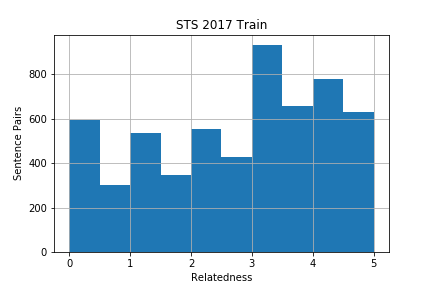
\includegraphics[width=\textwidth]{figures/semantic_textual_similarity/introduction/sts_train.png}
		\caption{Relatedness distribution of \\ STS 2017 training test}
		\label{fig:sts_train_relatedness}
	\end{subfigure}%
	\begin{subfigure}[b]{.5\textwidth}
		\centering
		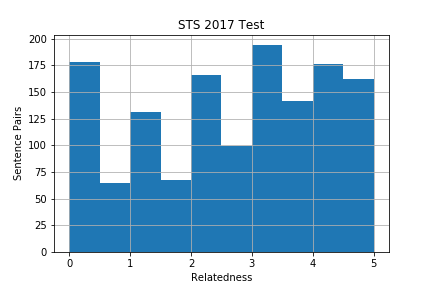
\includegraphics[width=\textwidth]{figures/semantic_textual_similarity/introduction/sts_test.png}
		\caption{Relatedness distribution of \\ STS 2017 testing set}
		\label{fig:sts_test_relatedness}
	\end{subfigure}
	\caption[Relatedness distribution of STS 2017 train and STS 2017 test]{Relatedness distribution of STS 2017 train and STS 2017 test. \textit{Sentence Pairs} shows the number of sentence pairs that a certain \textit{Relatedness bin} has.}
	\label{fig:sts_relatedness}
\end{figure}


\begin{figure}
	\captionsetup[subfigure]{justification=centering}
	\centering
	\begin{subfigure}[b]{.5\textwidth}
		\centering
		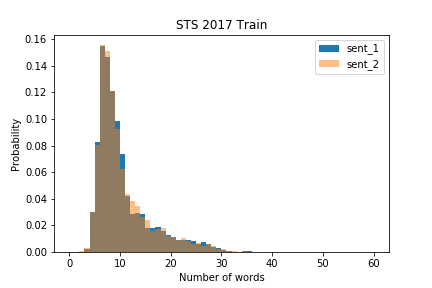
\includegraphics[width=\textwidth]{figures/semantic_textual_similarity/introduction/sts_2017_train_words.png}
		\caption{Normalised distribution of word count in STS 2017 train}
		\label{fig:sts_train_words}
	\end{subfigure}%
	\begin{subfigure}[b]{.5\textwidth}
		\centering
		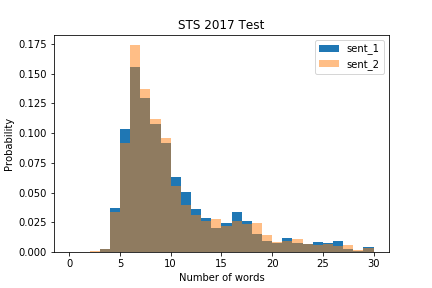
\includegraphics[width=\textwidth]{figures/semantic_textual_similarity/introduction/sts_2017_test_words.png}
		\caption{Normalised distribution of word count in STS 2017 test}
		\label{fig:sts_test_words}
	\end{subfigure}
	\caption[Normalised distribution of word count in STS 2017 train and STS 2017 test.]{Normalised distribution of word count in STS 2017 train and STS 2017 test. \textit{Number of words} indicates the word count and \textit{Probability} shows the total probability of a sentence with that word count appearing in the dataset.}
	\label{fig:sts_words}
\end{figure}

\begin{figure}
	\captionsetup[subfigure]{justification=centering}
	\centering
	\begin{subfigure}[b]{.5\textwidth}
		\centering
		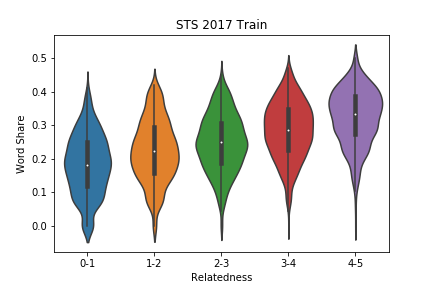
\includegraphics[width=\textwidth]{figures/semantic_textual_similarity/introduction/sts_2017_train_word_share.png}
		\caption{Word share against relatedness bins in STS 2017 train}
		\label{fig:sts_train_word_share}
	\end{subfigure}%
	\begin{subfigure}[b]{.5\textwidth}
		\centering
		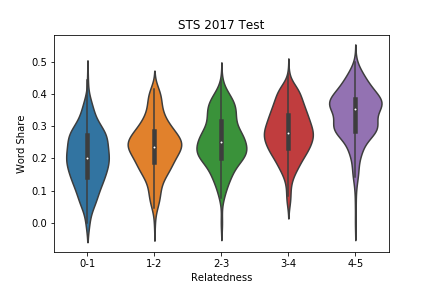
\includegraphics[width=\textwidth]{figures/semantic_textual_similarity/introduction/sts_2017_test_word_share.png}
		\caption{Word share against relatedness bins in STS 2017 test}
		\label{fig:sts_test_word_share}
	\end{subfigure}
	\caption[Word share against relatedness bins in STS 2017 train and STS 2017 test.]{Word share against relatedness bins in STS 2017 train and STS 2017 test. \textit{Word Share} indicates the ratio between number of common words in the two sentences to total number of words in the two sentences against each \textit{Relatedness} bins}
	\label{fig:sts_word_share}
\end{figure}


\begin{table*}
	\centering
	\begin{tabular}{l|cc|cc}
		\hline
		Measure   & \multicolumn{2}{c|}{STS 2017 Train} & \multicolumn{2}{c}{STS 2017 Test} \\
		\hline
		\multicolumn{1}{l|}{} & \textbf{Sent$\_$1} & \textbf{Sent$\_$2} & \textbf{Sent$\_$1} & \textbf{Sent$\_$2} \\
		\textit{Word Count Mean} & 10.01 & 9.94 & 9.83 & 9.80  \\
		\textit{Word Count STD} & 5.52 & 5.36 & 5.14 & 5.14  \\
		\textit{Word Count MAX} & 57 & 48 & 30 & 30  \\
		\textit{Word Count MIN} & 3 & 2 & 3 & 2  \\
		\hline
	\end{tabular}
	\caption[Word count stats in STS 2017]{Word count stats in STS 2017 training and STS 2017 testing.\textit{STD} indicates the standard deviation and the other acronyms indicate the common meaning }
	\label{table:sts_2017_sts}
\end{table*}

Similar to the SICK dataset, we calculate some statistics and produce some graphs. Figure \ref{fig:sts_relatedness} shows the relatedness distribution and Figure \ref{fig:sts_words} shows the normalised distribution of word count for sentence 1 and sentence 2 in STS 2017 train and test sets. Most of these statistics are similar to the SICK dataset. One notable change is the maximum word count in STS 2017 training dataset which is 57 in sentence 1 and 48 in sentence 2 according to Table \ref{table:sts_2017_sts} while both SICK datasets' and STS 2017 test set's maximum word count is limited to 30. We believe that the reason is STS train is composed with many sources including news articles which can have lengthy sentences. However, the STS algorithm should be able to properly handle this imbalance nature between STS2017 train and test set. 

In Figure \ref{fig:sts_word_share} we draw a violin plot for each relatedness score bin with word share. We can see that generally higher word share leads to higher relatedness, but still there can be sentence pairs contradicts this which is similar to the observation we had with SICK dataset. 

Since the statics of SICK and STS 2017 datasets are similar one dataset can be used to augment the training data in the other dataset which can lead to better results as neural networks perform better with more data \cite{wang-etal-2020-evaluating,info:doi/10.2196/23086}. We hope to experiment this with supervised machine learning models in Chapters \ref{cha:sts_siamese_neural_networks} and \ref{cha:sts_transformers}.
  
 \item \textbf{Quora Question Pairs} \footnote{The Quora Question Pairs Dataset is available to download at \url{http://qim.fs.quoracdn.net/quora_duplicate_questions.tsv}} The Quora Question Pairs dataset is a big dataset which was first released for a Kaggle Competition\footnote{Kaggle is an online community of data scientists and machine learning practitioners that hosts machine learning competitions. The Quora Question Pairs competition is available on \url{https://www.kaggle.com/c/quora-question-pairs}}. Quora is a question-and-answer website where questions are asked, answered, followed, and edited by internet users, either factually or in the form of opinions. If a particular new question has been asked before, users merge the new question to the original question flagging it as a duplicate. The organisers used this functionality to create the dataset and did not use a separate annotation process. Their original sampling method has returned an imbalanced dataset with many more true examples of duplicate pairs than non-duplicates. Therefore, the organisers have supplemented the dataset with negative examples. One source of negative examples 
 have been pairs of \textit{related question} which, although pertaining to similar topics, are not truly semantically equivalent. 
 
 The dataset has 400,000 question pairs and we used 4:1 split on that to separate it into a training set and a test set resulting 320,000 questions pairs in the training set and  80,000 sentence pairs in the testing set. The machine learning models need to predict a value between 0 and 1 that reflects whether it is a duplicate question pair or not. 1 indicates that a certain question pair is a duplicate and 0 indicates it is not a duplicate. 
 
    \begin{table}[ht!]
 	\centering 	
 	\begin{tabular}{l|c} 
 		\hline
 		\multicolumn{1}{c|}{\textbf{Question Pair}} & 
 		\multicolumn{1}{c}{\textbf{\detokenize{is-duplicate}}}  \\
 		\hline
 		\makecell[l]
 		{	1. What are natural numbers? \\ 
 			2. What is a least natural number?} & 0  \\
 		\hline
 		\makecell[l]
 		{	1. Which Pizzas are most popularly ordered \\ in Dominos menu? \\ 
 			2. How many calories does a Dominos Pizza have?} & 0  \\
 		\hline
 		\makecell[l]
 		{   1. How do you start a bakery? \\ 
 			2. How can one start a bakery business?} & 1  \\
 		\hline
 		\makecell[l]
 		{	1. Should I learn Python or Java first? \\ 
 			2. If I had to choose between learning \\ Java and Python what should I choose \\ to learn first?} & 1  \\
 		\hline
 		
 	\end{tabular}
 	\caption[Example question pairs from the Quora Question Pairs dataset]{Example question  pairs from the Quora Question Pairs dataset with their gold \detokenize{is-duplicate} value. \textbf{Question Pair} column shows the two questions and \textbf{is-duplicated} column denotes whether it is a duplicated pair or not.}
 	\label{tab:quoradata}
 \end{table}  


\begin{figure}
	\captionsetup[subfigure]{justification=centering}
	\centering
	\begin{subfigure}[b]{.5\textwidth}
		\centering
		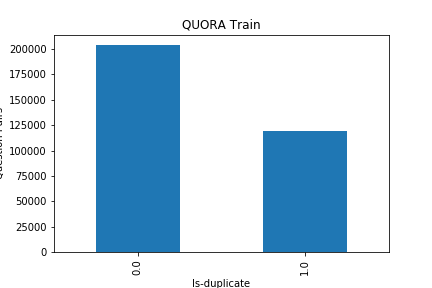
\includegraphics[width=\textwidth]{figures/semantic_textual_similarity/introduction/quora_train.png}
		\caption{Is-duplicate distribution of \\ QUORA training test}
		\label{fig:quora_train_is_duplicate}
	\end{subfigure}%
	\begin{subfigure}[b]{.5\textwidth}
		\centering
		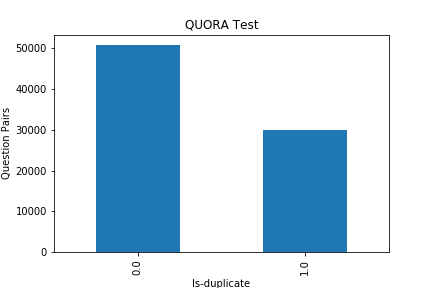
\includegraphics[width=\textwidth]{figures/semantic_textual_similarity/introduction/quora_test.png}
		\caption{Is-duplicate distribution of \\ QUORA testing set}
		\label{fig:quora_test_is_duplicate}
	\end{subfigure}
	\caption[Is-duplicate distribution of QUORA train and QUORA test]{Is-duplicate distribution of QUORA train and QUORA test. \textit{Sentence Pairs} shows the number of sentence pairs that a certain \textit{Is-duplicate} has.}
	\label{fig:quora_is_duplicate}
\end{figure}


\begin{figure}
	\captionsetup[subfigure]{justification=centering}
	\centering
	\begin{subfigure}[b]{.5\textwidth}
		\centering
		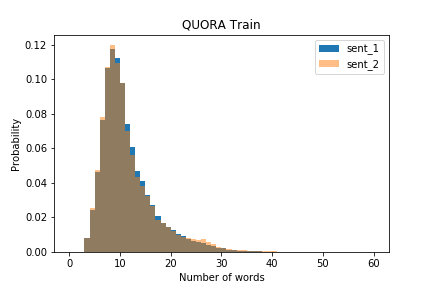
\includegraphics[width=\textwidth]{figures/semantic_textual_similarity/introduction/quora_train_words.png}
		\caption{Normalised distribution of word count in QUORA train}
		\label{fig:quora_train_words}
	\end{subfigure}%
	\begin{subfigure}[b]{.5\textwidth}
		\centering
		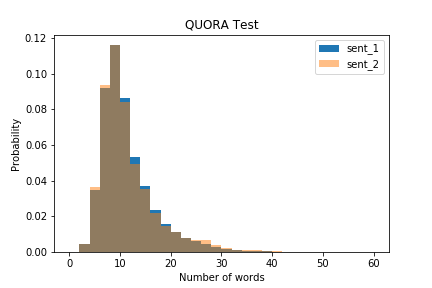
\includegraphics[width=\textwidth]{figures/semantic_textual_similarity/introduction/quora_test_words.png}
		\caption{Normalised distribution of word count in QUORA test}
		\label{fig:quora_test_words}
	\end{subfigure}
	\caption[Normalised distribution of word count in QUORA train and QUORA test.]{Normalised distribution of word count in QUORA train and QUORA test. \textit{Number of words} indicates the word count and \textit{Probability} shows the total probability of a sentence with that word count appearing in the dataset.}
	\label{fig:quora_words}
\end{figure}

\begin{figure}
	\captionsetup[subfigure]{justification=centering}
	\centering
	\begin{subfigure}[b]{.5\textwidth}
		\centering
		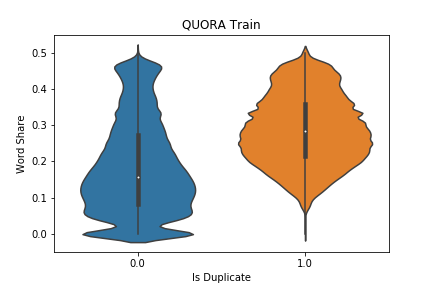
\includegraphics[width=\textwidth]{figures/semantic_textual_similarity/introduction/quora_train_word_share.png}
		\caption{Word share against is-relatedness value in QUORA train}
		\label{fig:quora_train_word_share}
	\end{subfigure}%
	\begin{subfigure}[b]{.5\textwidth}
		\centering
		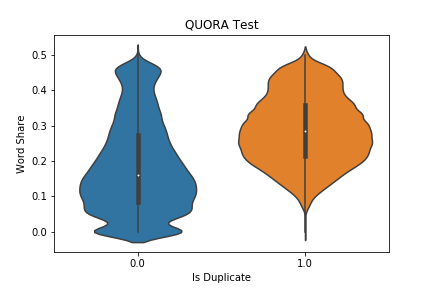
\includegraphics[width=\textwidth]{figures/semantic_textual_similarity/introduction/quora_test_word_share.png}
		\caption{Word share against is-relatedness value in QUORA test}
		\label{fig:quora_test_word_share}
	\end{subfigure}
	\caption[Word share against Is-duplicate values in QUORA train and QUORA test.]{Word share against Is-duplicate values in QUORA train and QUORA test. \textit{Word Share} indicates the ratio between number of common words in the two sentences to total number of words in the two sentences against each \textit{Is-duplicate}}
	\label{fig:quora_word_share}
\end{figure}


\begin{table*}
	\centering
	\begin{tabular}{l|cc|cc}
		\hline
		Measure   & \multicolumn{2}{c|}{QUORA Train} & \multicolumn{2}{c}{QUORA Test} \\
		\hline
		\multicolumn{1}{l|}{} & \textbf{Ques$\_$1} & \textbf{Ques$\_$2} & \textbf{Ques$\_$1} & \textbf{Ques$\_$2} \\
		\textit{Word Count Mean} & 10.95 & 11.20 & 10.92 & 11.14  \\
		\textit{Word Count STD} & 5.44 & 6.31 & 5.40 & 6.31  \\
		\textit{Word Count MAX} & 125 & 237 & 73 & 237  \\
		\textit{Word Count MIN} & 1 & 1 & 1 & 1  \\
		\hline
	\end{tabular}
	\caption[Word count stats in QUORA]{Word count stats in QUORA training and QUORA testing.\textit{STD} indicates the standard deviation and the other acronyms indicate the common meaning }
	\label{table:quora_sts}
\end{table*}
 
  
This is different to the previous datasets since it is not artificially created and use day to day language. Since it has more than 300,000 training instances deep learning systems will benefit more when used on this dataset. 

In Figure \ref{fig:quora_is_duplicate} we show the distribution of the two classes in QUORA dataset. The dataset seems to have more non duplicate question pairs than duplicate sentence pairs which is similar to the real world scenario. According to the word count distribution in Figure \ref{fig:quora_words} and word count statistics in Table \ref{table:quora_sts}, it is clear that QUORA datasets contains longer texts than SICK and STS 2017 datasets. Therefore, QUORA dataset should be able to test machine learning models'ability to handle lengthy texts properly. 

In Figure \ref{fig:quora_word_share} we show a violin plot for each \textit{"is-duplicate"} value with word share. We can see that duplicate questions have a high word share. However, it should be noted that there are non duplicate question pairs that still have a high word share. The machine learning algorithm should be able to handle them properly. 

According to statistics provided by the Director of Product Management at Quora on 17 September 2018, over 100 million people visit Quora every month, which raises the problem of different users asking similar questions with same intent but in different words \cite{8967103}. Multiple questions with the same intent can cause seekers to spend more time finding the best answer to their question, and make writers feel they need to answer multiple versions of the same question. Therefore, identifying duplicate questions will make it easier to find high quality answers to questions resulting in an improved experience for Quora writers, seekers, and readers.


\end{enumerate}

\subsection{Datasets on Other Languages}
One of the main requirements in our research was to build a STS method without depending on the language. Therefore through out our research we worked on several datasets from different languages. Those non-English datasets are described below. 
  
\begin{enumerate}
\item{ \textbf{Arabic STS Dataset \footnote{The Arabic STS dataset can be downloaded at \url{http://alt.qcri.org/semeval2017/task1/index.php?id=data-and-tools}}}} The Arabic STS dataset we selected was also used for the Arabic STS subtask in SemEval 2017 Task 1: Semantic Textual Similarity Multilingual and Cross-lingual Focused Evaluation \cite{cer-etal-2017-semeval}. Unlike Spanish, no data from previous SemEval competitions were available since this was the first time an Arabic STS task was organised in SemEval. More information about the extracted sentences will be shown in the Table \ref{tab:arabicdata_info}. 

\begin{table}[ht!]
	\centering
	\begin{tabular}{c|c|l}
		\hline
		\multicolumn{1}{c|}{\textbf{Dataset}} & 
		\multicolumn{1}{c|}{\textbf{Pairs}} & 
		\multicolumn{1}{c}{\textbf{Source}} \\
		\hline
		Trial & 23 & Mixed STS 2016 \\
		MSRpar  & 510 & newswire \\
		MSRvid  & 368 & videos \\
		SMTeuroparl  & 203 & WMT eval. \\
		\hline
	\end{tabular}
	\caption[Information about Arabic STS training set]{Information about the datasets used to build the Arabic STS training set. \textbf{Dataset} column expresses the acronym used describe the dataset. \textbf{Pairs} is the number of sentence pairs in that particular dataset and \textbf{Source} shows the source of the sentence pairs. }
	\label{tab:arabicdata_info}
\end{table}  

To prepare the annotated instances, a subset of the English STS 2017 dataset has been selected and human translated into Arabic. Sentences have been translated independently from their pairs. Arabic translation has been provided by native Arabic speakers with strong English skills in Carnegie Mellon University in Qatar. Translators have been given an English sentence and its Arabic machine translation5 where they have performed post-editing to correct errors. STS labels have been then transferred to the translated pairs. Therefore, annotation guidelines and the template will be similar to the English STS 2017 dataset. 1103 sentence pairs were available for training and 250 sentence pairs were available in the test set. Table \ref{tab:arabicdata} shows few pairs of sentences with their similarity score. The machine learning models require to predict a value between 0-5 which reflects the similarity of a given Arabic sentence pair. 

\begin{table}[ht!]
	\centering 	
	\begin{tabular}{l|c} 
		\hline
		\multicolumn{1}{c|}{\textbf{Sentence Pair}} & 
		\multicolumn{1}{c}{\textbf{\detokenize{Similarity}}}  \\
		\hline
		\makecell[l]
		{	1. \< أحدهم يقلي لحما.  > \\ \textit{Someone is frying meat.}\ \\ 
			2.  \< أحدهم يعزف البيانو.  > \\ \  \textit{Someone plays the piano.} } & 0.250
		\\
		\hline
		\makecell[l]
		{	1. \< أمرأة تظيف المكونات في الإناء.  > \\ \textit{
				A woman cleaning ingredients in the bowl.}\ \\ 
			2.  \< إمرأة تكسر ثلاثة بيضات في الإناء. > \\ \  \textit{
				A woman breaks three eggs in a bowl.} } & 1.750
		\\
		\hline
		\makecell[l]
		{	1. \< طفلة تعزف القيثارة.  > \\ \textit{A Child is playing harp.}\ \\ 
			2.  \< رجل يعزف القيثارة . > \\ \  \textit{A man plays the harp.} } & 2.250
		\\
		\hline
		\makecell[l]
		{	1. \< المرأة تقطع البصل الأخضر.  > \\ \textit{The woman chops green onions.}\ \\ 
			2.  \< إمرأة تقشر بصلة. > \\ \  \textit{A woman peeling an onion.} } & 3.250
		\\
		\hline
		\makecell[l]
		{	1. \< الأيل قفز فوق السياج. > \\ \textit{The deer jumped over the fence.}\ \\ 
			2.  \< أيل يقفز فوق سياج الإعصار. > \\ \  \textit{Deer Jumps Over Hurricane Fence} } & 4.800
		\\
		\hline
		
	\end{tabular}
	\caption[Example question pairs from the Arabic STS dataset]{Example question  pairs from the Arabic STS dataset. \textbf{Sentence Pair} column shows the two sentences. We also included their translations in the table. The translations were done by a native Arabic speaker. \textbf{Similarity} column indicates the annotated similarity of the two sentences.}
	\label{tab:arabicdata}
\end{table}  

\begin{figure}
	\captionsetup[subfigure]{justification=centering}
	\centering
	\begin{subfigure}[b]{.5\textwidth}
		\centering
		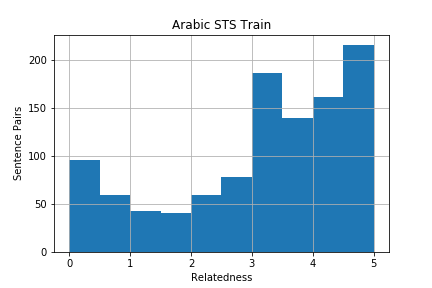
\includegraphics[width=\textwidth]{figures/semantic_textual_similarity/introduction/sts_arabic_train.png}
		\caption{Relatedness distribution of \\ Arabic STS  training test}
		\label{fig:arabic_train_relatedness}
	\end{subfigure}%
	\begin{subfigure}[b]{.5\textwidth}
		\centering
		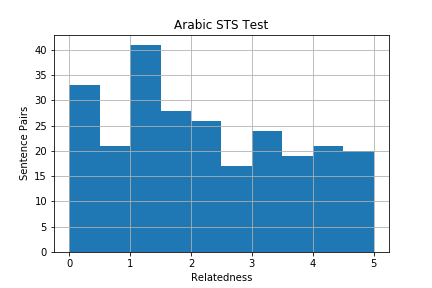
\includegraphics[width=\textwidth]{figures/semantic_textual_similarity/introduction/sts_arabic_test.png}
		\caption{Relatedness distribution of \\ Arabic STS  testing set}
		\label{fig:arabic_test_relatedness}
	\end{subfigure}
	\caption[Relatedness distribution of Arabic STS train and Arabic STS test]{Relatedness distribution of Arabic STS train and Arabic STS test. \textit{Sentence Pairs} shows the number of sentence pairs that a certain \textit{Relatedness bin} has.}
	\label{fig:arabic_sts_relatedness}
\end{figure}


\begin{figure}
	\captionsetup[subfigure]{justification=centering}
	\centering
	\begin{subfigure}[b]{.5\textwidth}
		\centering
		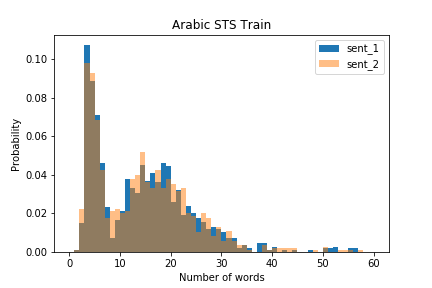
\includegraphics[width=\textwidth]{figures/semantic_textual_similarity/introduction/arabic_sts_train_words.png}
		\caption{Normalised distribution of word count in Spanish STS train}
		\label{fig:arabic_sts_train_words}
	\end{subfigure}%
	\begin{subfigure}[b]{.5\textwidth}
		\centering
		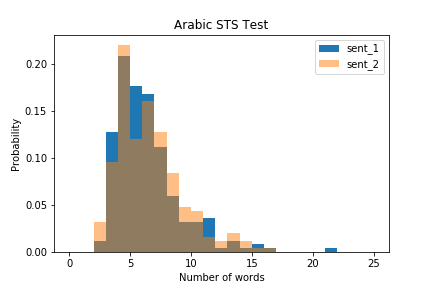
\includegraphics[width=\textwidth]{figures/semantic_textual_similarity/introduction/arabic_sts_test_words.png}
		\caption{Normalised distribution of word count in Spanish STS test}
		\label{fig:arabic_sts_test_words}
	\end{subfigure}
	\caption[Normalised distribution of word count in Arabic STS train and Arabic STS test.]{Normalised distribution of word count in Arabic STS train and Arabic STS test. \textit{Number of words} indicates the word count and \textit{Probability} shows the total probability of a sentence with that word count appearing in the dataset.}
	\label{fig:arabic_sts_words}
\end{figure}

\begin{figure}
	\captionsetup[subfigure]{justification=centering}
	\centering
	\begin{subfigure}[b]{.5\textwidth}
		\centering
		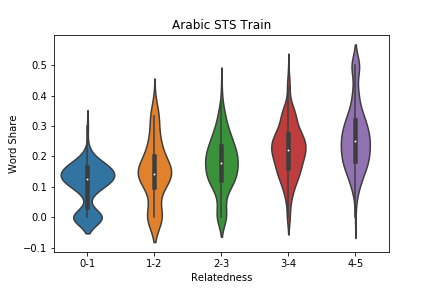
\includegraphics[width=\textwidth]{figures/semantic_textual_similarity/introduction/arabic_sts_train_word_share.png}
		\caption{Word share against relatedness bins in Arabic STS train}
		\label{fig:arabic_sts_train_word_share}
	\end{subfigure}%
	\begin{subfigure}[b]{.5\textwidth}
		\centering
		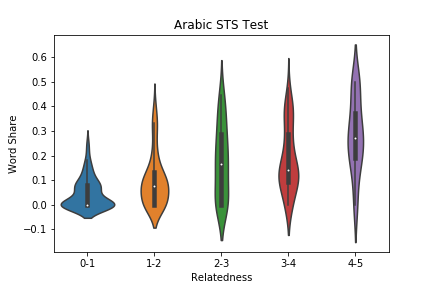
\includegraphics[width=\textwidth]{figures/semantic_textual_similarity/introduction/arabic_sts_test_word_share.png}
		\caption{Word share against relatedness bins in Arabic STS test}
		\label{fig:arabic_sts_test_word_share}
	\end{subfigure}
	\caption[Word share against relatedness bins in Arabic STS train and Arabic STS test.]{Word share against relatedness bins in Arabic STS train and Spanish STS test. \textit{Word Share} indicates the ratio between number of common words in the two sentences to total number of words in the two sentences against each \textit{Relatedness} bins}
	\label{fig:arabic_sts_word_share}
\end{figure}


\begin{table*}
	\centering
	\begin{tabular}{l|cc|cc}
		\hline
		Measure   & \multicolumn{2}{c|}{Spanish STS Train} & \multicolumn{2}{c}{Spanish STS Test} \\
		\hline
		\multicolumn{1}{l|}{} & \textbf{Sent$\_$1} & \textbf{Sent$\_$2} & \textbf{Sent$\_$1} & \textbf{Sent$\_$2} \\
		\textit{Word Count Mean} & 31.23 & 31.02 & 9.03 & 9.34  \\
		\textit{Word Count STD} & 12.15 & 12.37 & 3.66 & 3.74  \\
		\textit{Word Count MAX} & 90 & 90 & 22 & 24  \\
		\textit{Word Count MIN} & 5 & 1 & 3 & 3  \\
		\hline
	\end{tabular}
	\caption[Word count stats in Arabic STS]{Word count stats in Arabic STS training and Arabic STS testing.\textit{STD} indicates the standard deviation and the other acronyms indicate the common meaning }
	\label{table:arabic_sts}
\end{table*}	
	

\item{ \textbf{Spanish STS Dataset \footnote{The Spanish STS dataset can be downloaded at \url{http://alt.qcri.org/semeval2017/task1/index.php?id=data-and-tools}}}} - Spanish STS dataset that we used was employed for Spanish STS subtask in SemEval 2017 Task 1: Semantic Textual Similarity Multilingual and Cross-lingual Focused Evaluation \cite{cer-etal-2017-semeval}. The training set has 1250 sentence pairs annotated with a relatedness score between 0 and 4. The training set combined several datasets from previous SemEval STS shared tasks also\cite{cer-etal-2017-semeval}. Table \ref{tab:spanishdata_info} shows more information about the training set. There were two sources for test set - Spanish news and Spanish Wikipedia dump having 500 and 250 sentence pairs respectively \cite{cer-etal-2017-semeval}. Both datasets were annotated with a relatedness score between 0 and 5. Table \ref{tab:spanishdata} shows few pairs of sentences with their similarity score. The machine learning models require to predict a value between 0-5 which reflects the similarity of the given Spanish sentence pair.

\begin{table}[ht!]
	\centering
	\begin{tabular}{c|c|c|l}
		\hline
		\multicolumn{1}{c|}{\textbf{Year}} & 
		\multicolumn{1}{c|}{\textbf{Dataset}} & 
		\multicolumn{1}{c|}{\textbf{Pairs}} & 
		\multicolumn{1}{c}{\textbf{Source}} \\
		\hline
		 & Trial & 56 & NR \\
		2014 \cite{agirre-etal-2014-semeval} & Wiki  & 324 & Spanish Wikipedia \\
		 & News  & 480 & Newswire \\
		\hline
		2015 \cite{agirre-etal-2014-semeval} & Wiki & 251 & Spanish Wikipedia \\
		 & News & 500 & Sewswire \\
		\hline
	\end{tabular}
	\caption[Information about Spanish STS training set]{Information about the datasets used to build the Spanish STS training set. The \textbf{Year} column shows the year of the SemEval competition that the dataset got released. \textbf{Dataset} column expresses the acronym used describe a dataset in that year. \textbf{Pairs} is the number of sentence pairs in that particular dataset and \textbf{Source} shows the source of the sentence pairs. }
	\label{tab:spanishdata_info}
\end{table}


\begin{table}[ht!]
	\centering
		\begin{tabular}{l|c}
			\hline
			\multicolumn{1}{c|}{\textbf{Sentence Pair}} & 
			\multicolumn{1}{c}{\textbf{Similarity}}  \\
			\hline
			\makecell[l]{1. Amás, los misioneros apunten que los númberos \\ d'infectaos puen ser shasta dos o hasta cuatro veces \\ más grandess que los oficiales. \\
				\textit{(Furthermore, missionaries point out that the numbers of } \\ \textit{infected can be up to two or up to four times larger than} \\ \textit{the official ones.)} \\ 
				2. Los cadáveres de personas fallecidas pueden ser hasta \\ diez veces más contagiosos que los infectados vivos. \\ 
			\textit{(The corpses of deceased people can be up to ten times } \\ \textit{more contagious than those infected alive.)}} & 0.6  \\
%			\hline
%			\makecell[l]{1. Desde Colombia, el presidente Juan Manuel Santos dijo \\ que conversó por teléfono con Humala sobre el tema y que \\ entregaría al detenido a las autoridades peruanas a más tardar \\ el viernes. \\ 
%				\textit{(From Colombia, President Juan Manuel Santos said he spoke} \\ \textit{by phone with Humala about the matter and that he would hand} \\ \textit{over the detainee to the Peruvian authorities no later than Friday.)}\\
%				2. El presidente de Colombia, Juan Manuel Santos, había \\ anunciado horas antes que Orellana, que se encuentra \\ detenido, será entregado a las autoridades peruanas sentre \\ hoy y mañanas. \\
%			   \textit{(The president of Colombia, Juan Manuel Santos, had announced} \\ \textit{hours before that Orellana, who is in detention, will be handed over} \\ \textit{to the Peruvian authorities today and tomorrow.)}}  
%			 & 3.2 \\
			\hline
			\makecell[l]{1. La policía abatió a un caníbal cuando devoraba a una  \\ mujer Matthew Williams, de 34 años, fue sorprendido en \\ la madrugada mordiendo el rostro de una joven a la que  \\ había invitado a su hotel. \\ 
				\textit{(Police killed a cannibal while devouring a woman Matthew } \\ \textit{Williams, 34, was caught early in the morning biting the} \\ \textit{ face of a young woman he had invited to his hotel.)} \\
				2. La policía de Gales del Sur mató a un caníbal cuando se \\ estaba comiendo la cara de una mujer de 22 años en la \\ habitación de un hotel. \\ 
			\textit{(South Wales police killed a cannibal when he was eating the } \\ \textit{face of a 22-year-old woman in a hotel room.)} } & 2  \\
			\hline
			\makecell[l]{1. Ollanta Humala se reúne mañana con el Papa Francisco. \\
				\textit{(Ollanta Humala meets tomorrow with Pope Francis.)} \\ 
				2. El Papa Francisco mantuvo hoy una audiencia privada \\ con el presidente Ollanta Humala, en el Vaticano. \\
			\textit{(Pope Francis held a private audience today with President} \\ \textit{Ollanta Humala, at the Vatican.)}} & 3  \\
			\hline               
		\end{tabular}
	\caption[Example sentence pairs from the Spanish STS dataset]{Example sentence pairs from the Spanish STS dataset. \textbf{Sentence Pair} column shows the two sentences. We also included their translations in the table. The translations were done by a native Spanish speaker. \textbf{Similarity} column indicates the annotated similarity of the two sentences. }
	\label{tab:spanishdata}
\end{table}  

\begin{figure}
	\captionsetup[subfigure]{justification=centering}
	\centering
	\begin{subfigure}[b]{.5\textwidth}
		\centering
		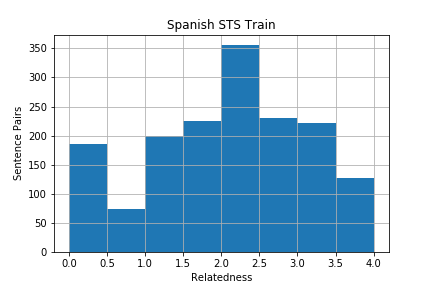
\includegraphics[width=\textwidth]{figures/semantic_textual_similarity/introduction/sts_spanish_train.png}
		\caption{Relatedness distribution of \\ Spanish STS  training test}
		\label{fig:spanish_train_relatedness}
	\end{subfigure}%
	\begin{subfigure}[b]{.5\textwidth}
		\centering
		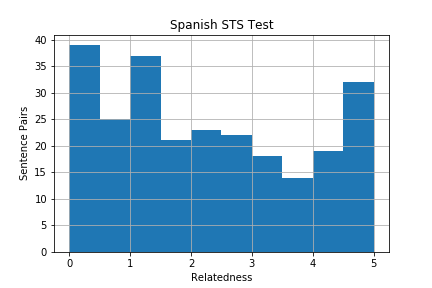
\includegraphics[width=\textwidth]{figures/semantic_textual_similarity/introduction/sts_spanish_test.png}
		\caption{Relatedness distribution of \\ Spanish STS  testing set}
		\label{fig:spanish_test_relatedness}
	\end{subfigure}
	\caption[Relatedness distribution of Spanish STS train and Spanish STS test]{Relatedness distribution of Spanish STS train and Spanish STS test. \textit{Sentence Pairs} shows the number of sentence pairs that a certain \textit{Relatedness bin} has.}
	\label{fig:spanish_sts_relatedness}
\end{figure}


\begin{figure}
	\captionsetup[subfigure]{justification=centering}
	\centering
	\begin{subfigure}[b]{.5\textwidth}
		\centering
		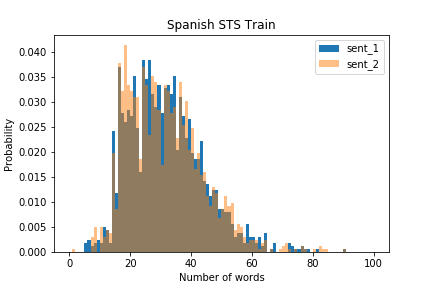
\includegraphics[width=\textwidth]{figures/semantic_textual_similarity/introduction/spanish_sts_train_words.png}
		\caption{Normalised distribution of word count in Spanish STS train}
		\label{fig:spanish_sts_train_words}
	\end{subfigure}%
	\begin{subfigure}[b]{.5\textwidth}
		\centering
		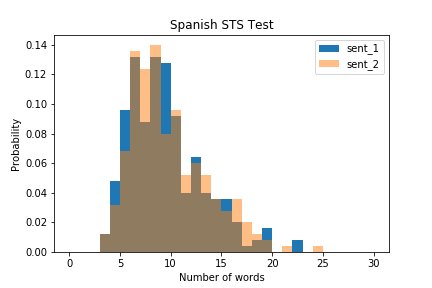
\includegraphics[width=\textwidth]{figures/semantic_textual_similarity/introduction/spanish_sts_test_words.png}
		\caption{Normalised distribution of word count in Spanish STS test}
		\label{fig:spanish_sts_test_words}
	\end{subfigure}
	\caption[Normalised distribution of word count inSpanish STS train and Spanish STS test.]{Normalised distribution of word count in Spanish STS train and Spanish STS test. \textit{Number of words} indicates the word count and \textit{Probability} shows the total probability of a sentence with that word count appearing in the dataset.}
	\label{fig:spanish_sts_words}
\end{figure}

\begin{figure}
	\captionsetup[subfigure]{justification=centering}
	\centering
	\begin{subfigure}[b]{.5\textwidth}
		\centering
		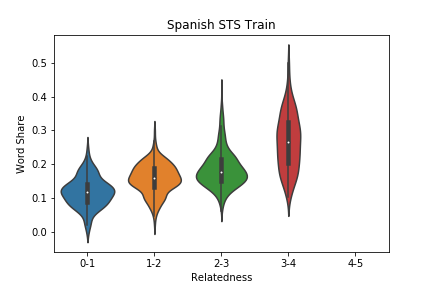
\includegraphics[width=\textwidth]{figures/semantic_textual_similarity/introduction/spanish_sts_train_word_share.png}
		\caption{Word share against relatedness bins in Spanish STS train}
		\label{fig:spanish_sts_train_word_share}
	\end{subfigure}%
	\begin{subfigure}[b]{.5\textwidth}
		\centering
		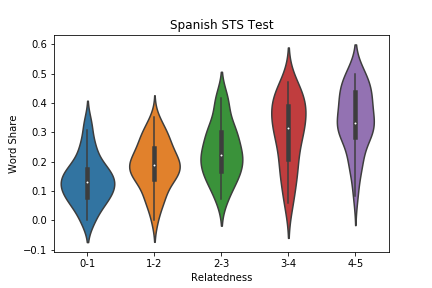
\includegraphics[width=\textwidth]{figures/semantic_textual_similarity/introduction/spanish_sts_test_word_share.png}
		\caption{Word share against relatedness bins in Spanish STS test}
		\label{fig:spanish_sts_test_word_share}
	\end{subfigure}
	\caption[Word share against relatedness bins in Spanish STS train and STS 2017 test.]{Word share against relatedness bins in Spanish STS train and Spanish STS test. \textit{Word Share} indicates the ratio between number of common words in the two sentences to total number of words in the two sentences against each \textit{Relatedness} bins}
	\label{fig:spanish_sts_word_share}
\end{figure}


\begin{table*}
	\centering
	\begin{tabular}{l|cc|cc}
		\hline
		Measure   & \multicolumn{2}{c|}{Spanish STS Train} & \multicolumn{2}{c}{Spanish STS Test} \\
		\hline
		\multicolumn{1}{l|}{} & \textbf{Sent$\_$1} & \textbf{Sent$\_$2} & \textbf{Sent$\_$1} & \textbf{Sent$\_$2} \\
		\textit{Word Count Mean} & 31.23 & 31.02 & 9.03 & 9.34  \\
		\textit{Word Count STD} & 12.15 & 12.37 & 3.66 & 3.74  \\
		\textit{Word Count MAX} & 90 & 90 & 22 & 24  \\
		\textit{Word Count MIN} & 5 & 1 & 3 & 3  \\
		\hline
	\end{tabular}
	\caption[Word count stats in Spanish STS]{Word count stats in Spanish STS training and Spanish STS testing.\textit{STD} indicates the standard deviation and the other acronyms indicate the common meaning }
	\label{table:spanish_sts}
\end{table*}

Similar to the English datasets we calculate some statistics and produce some graphs. A key challenge in the Spanish STS dataset is that test set is very different from the training set. As can be seen in Figure \ref{fig:spanish_sts_relatedness} training set has been annotated with relatedness scores 0-4 while the test set has been annotated with relatedness scores 0-5. Therefore, STS methods should be able to handle that properly. Furthermore, as shown in Figure \ref{fig:spanish_sts_words} and in Table \ref{table:spanish_sts} sentence pairs in test set are shorter in word length than the sentence pairs in train set. Therefore, STS methods working on this dataset should be able to properly handle that too. This can be observed as a weakness in this dataset, but at the same time this property of the dataset can be exploited to measure the strength of a STS system as well.

	


	
\end{enumerate}


\subsection{Datasets on Different Domains}
In order to experiment how our STS methods can be adopted in to different domains we also used a dataset from a different discipline which we introduce in this section. 
\begin{enumerate}
	
	\item{ \textbf{Bio-medical STS Dataset: BIOSSES } \footnote{Bio-medical STS Dataset: BIOSSES  can be downloaded from \url{https://tabilab.cmpe.boun.edu.tr/BIOSSES/DataSet.html} }} - BIOSSES is the first and only benchmark dataset for biomedical  sentence  similarity  estimation.
	\cite{10.1093/bioinformatics/btx238}. The  dataset  comprises 100 sentence pairs, in which each sentence has been selected from the TAC (Text Analysis Conference) Biomedical Summarisation Track- training dataset containing articles from  the  biomedical domain \footnote{Biomedical Summarisation Track is a shared task organised in TAC 2014 - \url{https://tac.nist.gov/2014/BiomedSumm/}}. The sentence pairs have been evaluated by five different human experts that judged their similarity and gave scores ranging from 0 (no relation) to 4 (equivalent). The score range was described based on the guidelines of SemEval 2012 Task 6 on STS \cite{agirre-etal-2012-semeval}. Besides the annotation instructions, example sentences from the bio-medical literature have been also provided to the annotators for each of the similarity degrees. To represent the similarity between two sentences we took the average of the scores provided by the five human experts. Table \ref{tab:biomeddata} shows few examples in the dataset. The machine learning models require to predict a value between 0-4 which reflects the similarity of the given bio medical sentence pair.
	
	A dataset as small as this one can not be used by to train a supervised ML method, requiring alternative approaches such as unsupervised methods and transfer learning techniques which we will be exploring in the next few chapters.
	
	\begin{table}[ht!]
		\centering
			\begin{tabular}{c|c}
				\hline
				\multicolumn{1}{c|}{\textbf{Sentence Pair}} & 
				\multicolumn{1}{c}{\textbf{Similarity}}  \\
				\hline
				\makecell[l]{1. It has recently been shown that Craf is essential \\ for Kras G12D-induced NSCLC. \\ 
					2. It has recently become evident that Craf is \\ essential for the onset of Kras-driven non-small \\ cell lung cancer.} & 4  \\
				\hline
				\makecell[l]{1. Up-regulation of miR-24 has been observed in \\ a number of cancers, including OSCC. \\ 
					2. In addition, miR-24 is one of the most abundant \\ miRNAs in cervical cancer cells, and is reportedly \\ up-regulated in solid stomach cancers. } & 3 \\
				\hline
				\makecell[l]{1. These cells (herein termed TLM-HMECs) are \\ immortal but do not proliferate in the absence of \\ extracellular matrix (ECM) \\  
					2. HMECs expressing hTERT and SV40 LT \\ (TLM-HMECs) were cultured in mammary epithelial \\ growth medium (MEGM, Lonza)  } & 1.4  \\
				\hline
				\makecell[l]{1.The up-regulation of miR-146a was also detected in \\ cervical cancer tissues.  \\ 
					2. Similarly to PLK1, Aurora-A activity is required \\ for the enrichment or localisation of multiple \\ centrosomal  factors which have roles in maturation, \\ including LATS2 and CDK5RAP2/Cnn.} & 0.2  \\
				\hline               
			\end{tabular}
		\caption[Example question pairs from the BIOSSES dataset]{Example question  pairs from the BIOSSES dataset. \textbf{Sentence Pair} column shows the two sentences. \textbf{Similarity} column indicates the averaged annotated similarity of the two sentences.}
		\label{tab:biomeddata}
	\end{table} 

\begin{figure}
	\centering
	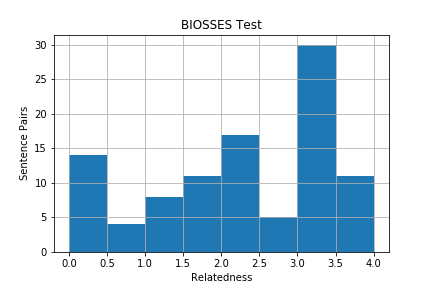
\includegraphics[width=0.8\textwidth]{figures/semantic_textual_similarity/introduction/biosses.png}
	\caption[Relatedness distribution of BIOSSES]{Relatedness distribution of BIOSSES. \textit{Sentence Pairs} shows the number of sentence pairs that a certain \textit{Relatedness bin} has.}
	\label{fig:biosses_relatedness}
\end{figure}

\begin{figure}
	\centering
	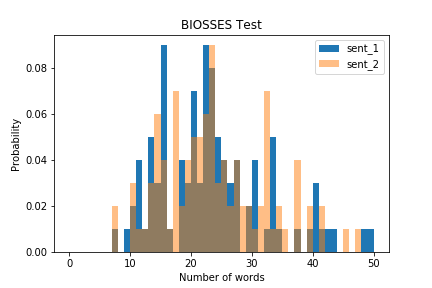
\includegraphics[width=0.8\textwidth]{figures/semantic_textual_similarity/introduction/biosses_words.png}
	\caption[Normalised distribution of word count in BIOSSES.]{Normalised distribution of word count in BIOSSES. \textit{Number of words} indicates the word count and \textit{Probability} shows the total probability of a sentence with that word count appearing in the dataset.}
	\label{fig:biosses_words}
\end{figure}


\begin{figure}
	\centering
	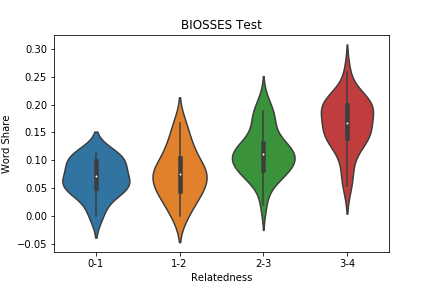
\includegraphics[width=0.8\textwidth]{figures/semantic_textual_similarity/introduction/biosses_word_share.png}
	\caption[Word share against relatedness bins in BIOSSES.]{Word share against relatedness bins in BIOSSES. \textit{Word Share} indicates the ratio between number of common words in the two sentences to total number of words in the two sentences against each \textit{Relatedness} bins}
	\label{fig:biosses_word_share}
\end{figure}

\end{enumerate}

\section{Evaluation Metrics}
\label{sec:sts_evaluation}
While training a model is a key step, how the model generalises on unseen data is an equally important aspect that should be considered in every machine learning model. We need to know whether it actually works and, consequently, if we can trust its predictions. This is typically called as \textit{evaluation}. All of the datasets that we introduced in the previous section has what we call a \textit{test} set. The machine learning models need to provide their predictions for the test set and the predictions will be evaluated against the true values of the test set. 

There are three common evaluation metrics that are employed in Semantic Textual Similarity tasks, which we explain in this section. We will be using them to evaluate our models through out the first part of our research. 

In the equations presented for each of the evaluation metrics, we represent the gold labels with $X$ and predictions with $Y$. Therefore, a gold label in $i^{th}$ position will be represented by $X_i$ and a prediction in $i^{th}$ position will be represented by $Y_i$. 

\begin{enumerate}
	
	\item \textbf{Pearson's Correlation Coefficient} - Correlation is a technique for investigating the relationship between two quantitative, continuous variables. Pearson's correlation coefficient ($\rho$)  is a measure of the strength of the linear association between the two variables. A value of +1 is total positive linear correlation between the variables, 0 is no linear correlation, and -1 is total negative linear correlation. 
	
	Pearson's Correlation Coefficient is one of the most common evaluation metrics in STS shared tasks \cite{marelli-etal-2014-semeval,agirre-etal-2012-semeval,agirre-etal-2013-sem,agirre-etal-2014-semeval,agirre-etal-2015-semeval,agirre-etal-2016-semeval}. A machine learning model with a Pearson's Correlation Coefficient close to 1 indicates that the predictions of that model and gold labels have a strong positive linear correlation and therefore, it is a good model to predict STS. Pearson's Correlation Coefficient equation is shown in Equation \ref{equ:pearson} where $cov$  is the covariance, $\sigma_X$ is the standard deviation of $X$ and $\sigma_Y$ is the standard deviation of $Y$.
	
	\begin{equation}
	\label{equ:pearson}
	\rho = \frac{\text{cov}(X,Y)}{\sigma_X \sigma_Y}
	\end{equation}
	
	\item \textbf{Spearman's Correlation Coefficient} - Spearman's Correlation Coefficient ($\tau$) is another common evaluation metric in STS shared tasks \cite{marelli-etal-2014-semeval,agirre-etal-2012-semeval,agirre-etal-2013-sem,agirre-etal-2014-semeval,agirre-etal-2015-semeval,agirre-etal-2016-semeval}. It assesses how well the relationship between two variables can be described using a monotonic function. A monotonic relationship is a relationship that does one of the following: 
	
	\begin{enumerate}
		\item as the value of one variable increases, so does the value of the other variable, \textit{OR},
		\item as the value of one variable increases, the other variable value decreases.
	\end{enumerate}
	
	But not exactly at a constant rate whereas in a linear relationship the rate of increase/decrease is constant. The fundamental difference between Pearson's Correlation Coefficient and Spearman's Correlation Coefficient is that the Pearson Correlation Coefficient only works with a linear relationship between the two variables whereas the Correlation Coefficient works with the monotonic relationships as well. Spearman's Correlation Coefficient equation is shown in Equation \ref{equ:spearman} where $D_i$ is the pairwise distances of the ranks of the variables $X_i$ and $Y_i$ and $n$ is the number of elements in $X$ or $Y$.  
	
	
	\begin{equation}
	\label{equ:spearman}
	\tau = 1- {\frac {6 \sum D_i^2}{n(n^2 - 1)}}
	\end{equation}
	
	
	\item \textbf{Root Mean Squared Error} - Both Pearson's Correlation Coefficient and Spearman's Correlation Coefficient works only when both gold labels($X$) and predictions ($Y$) are continues. Therefore, in the datasets like Quora Question Pairs where the gold labels are discrete values, Root Mean Squared Error (RMSE) is preferred for evaluation than Correlation Coefficient values. RMSE measures the distance between the gold labels and the predictions. RMSE equation is shown in Equation \ref{equ:rmse} where $n$ is the number of elements in $X$ or $Y$. 
	
	\begin{equation}
	\label{equ:rmse}
	rmse = \sqrt{(\frac{1}{n})\sum_{i=1}^{n}(Y_{i} - X_{i})^{2}}
	\end{equation}
	
\end{enumerate}

\section{Conclusion}
Calculating the STS is an important research area in NLP which plays a vital role in many applications such as question answering, document summarisation, information retrieval and information extraction. Most of the early approaches were based on traditional machine learning and involved heavy feature engineering. However these approaches are difficult to be adopted in different languages and do not provide competitive results any more. With the advances of word embeddings, and as a result of the success neural networks have achieved in other fields, most of the methods proposed in recent years rely on word vectors. These methods can be further categorised in to supervised and unsupervised methods. Analysing STS methods belong to both of these categories would be beneficial to the community. Furthermore, exploring the ability of these methods to perform in a multilingual setting and a multi-domain setting would a timely contribution to the NLP field. 

The introduction of competitive STS shared tasks led to the development of standard datasets. From the publicly available datasets we selected three recently released English STS datasets; SICK, STS2017 and Quora Question Pairs. They carry different characteristics. We exploratory analysed these dataset focussing on common properties like size of the dataset, sentence length, common number of words etc. Furthermore, we identified certain properties of these datasets that would limit the performance of traditional STS methods like edit distance. For the multilingual experiments we selected a Spanish and an Arabic dataset. Similar to the English STS datasets we exploratory analysed them for certain characteristics. For the multi-domain experiments, we selected a Bio-medical STS Dataset. This dataset bring a key challenge to the STS methods as it does not have a separate training set. Therefore, this dataset would provide the opportunity to evaluate various STS methods in an out-of-domain and unsupervised setting.

The STS shared tasks has further contributed to the development of evaluation measures in STS. In all the datasets except Quora Question Pairs, Pearson Correlation and Spearman Correlation has been used to evaluate STS methods and in Quora dataset, Root Mean Squared Error has been used to evaluate the methods. We followed the same evaluation measures in order to compare our methods with other systems submitted the competition. 

In the next few chapters we will be exploring different unsupervised and supervised STS methods. We will be evaluating them in English STS datasets, non-English STS datasets as well as out of domain STS datasets to investigate their adaptability in different environments.

   


